\documentclass[aspectratio=169,10pt]{beamer}

\usetheme{Madrid}
\usecolortheme{seahorse}
\useinnertheme{rectangles}

\usepackage[utf8]{inputenc}
\usepackage{amsmath,amssymb,amsfonts}
\usepackage{mathtools}
\usepackage{xcolor}
\usepackage{graphicx}
\usepackage{booktabs}
\usepackage{array}

% Set graphicspath
\graphicspath{{figures/}}

% Code listing style (commented out - using verbatim instead)
%\lstset{
%    language=Python,
%    basicstyle=\ttfamily\scriptsize,
%    keywordstyle=\color{blue},
%    commentstyle=\color{gray},
%    stringstyle=\color{red},
%    breaklines=true,
%    showstringspaces=false,
%    numbers=left,
%    numberstyle=\tiny\color{gray},
%    frame=single,
%    rulecolor=\color{black},
%    backgroundcolor=\color{white!95!gray}
%}

% Custom commands
\newcommand{\gra}{\mathrm{gra}\;}
\newcommand{\dom}{\mathrm{dom}\;}
\newcommand{\ran}{\mathrm{ran}\;}
\newcommand{\Id}{\mathrm{Id}}
\newcommand{\Prox}{\mathrm{Prox}}
\newcommand{\sgn}{\mathrm{sgn}}
\newcommand{\inprod}[2]{\langle #1 \mid #2 \rangle}
\newcommand{\norm}[1]{\left\|#1\right\|}
\newcommand{\abs}[1]{\left|#1\right|}
\newcommand{\set}[1]{\left\{#1\right\}}
\newcommand{\Hilbert}{\mathcal{H}}
\newcommand{\Reals}{\mathbb{R}}
\newcommand{\argmin}{\operatornamewithlimits{arg\,min}}
\newcommand{\interior}{\mathrm{int}\;}
\newcommand{\cl}{\mathrm{cl}\;}

% Title page content
\title{Chapter 20: Monotone Operators}
\subtitle{Convex Analysis and Monotone Operator Theory in Hilbert Spaces, 2nd Edition}
\author{Bauschke \& Combettes (2017)}
\date{}
\institute{Based on Convex Analysis and Monotone Operator Theory}

\setbeamertemplate{footline}[frame number]
\setbeamertemplate{navigation symbols}{}

\begin{document}

\frame{\titlepage}

% ============================================================================
% Overview Frame
% ============================================================================
\begin{frame}
    \frametitle{Chapter 20: Overview}

    \begin{columns}[T]
        \column{0.5\textwidth}
        \textbf{Main Topics:}
        \begin{itemize}
            \item[\textcolor{blue}{\(\checkmark\)}] Monotone operators: Definition and examples
            \item[\textcolor{blue}{\(\checkmark\)}] Maximally monotone operators
            \item[\textcolor{blue}{\(\checkmark\)}] The partial inverse
            \item[\textcolor{blue}{\(\checkmark\)}] Bivariate functions and maximal monotonicity
            \item[\textcolor{blue}{\(\checkmark\)}] The Fitzpatrick function
        \end{itemize}

        \column{0.5\textwidth}
        \textbf{Key Results:}
        \begin{itemize}
            \item Moreau's Theorem
            \item Zorn's Lemma (existence of max. extensions)
            \item Spingarn's Proposition
            \item Rockafellar's Proposition
            \item Minty's Theorem (Ch. 21)
        \end{itemize}
    \end{columns}

    \vspace{2em}
    \centering
    \textit{Monotone operators form the foundation of modern optimization algorithms and variational analysis.}
\end{frame}

% ============================================================================
% Section 20.1: Monotone Operators
% ============================================================================
\section{20.1 Monotone Operators}

\begin{frame}
    \frametitle{Definition: Monotone Operator}

    \begin{definition}[Definition 20.1]
        Let $A : \Hilbert \to 2^{\Hilbert}$ be a set-valued operator. Then $A$ is \textbf{monotone} if
        \[
            (\forall (x,u) \in \gra A)(\forall (y,v) \in \gra A) \quad
            \inprod{x - y}{u - v} \geq 0.
        \]
    \end{definition}

    \vspace{1em}

    \begin{itemize}
        \item The condition says: vectors in the graph maintain non-negative inner products
        \item This is weaker than monotonicity for single-valued operators
        \item For single-valued $A : \Hilbert \to \Hilbert$: monotone iff $\inprod{x-y}{Ax-Ay} \geq 0$
    \end{itemize}

    \vspace{1.5em}

    \begin{example}[Basic Properties]
        For monotone $A$:
        \begin{enumerate}
            \item[(i)] $\inprod{x - y}{u - v} \geq 0$ for all $(x,u), (y,v) \in \gra A$
            \item[(ii)] Monotonicity extends to pairs with identical first or second component
            \item[(iii)] Key inequality: $\norm{u - v}^2 + \norm{x - y}^2 \geq \norm{x - y}^2 + \norm{u - v}^2$
        \end{enumerate}
    \end{example}
\end{frame}

\begin{frame}
    \frametitle{Examples of Monotone Operators}

    \begin{example}[Example 20.3: Subdifferential]
        If $f : \Hilbert \to \left]-\infty, +\infty\right]$ is proper and convex, then $\partial f$ is monotone.

        \textit{Proof:} By the subdifferential inequality: $\inprod{x-y}{u-v} \geq 0$ follows from the property that
        for $(x,u), (y,v) \in \gra \partial f$, we have $\inprod{x-y \mid u} \geq f(x) - f(y)$ and
        $\inprod{y-x \mid v} \geq f(y) - f(x)$. Adding these yields the result.
    \end{example}

    \vspace{1em}

    \begin{example}[Example 20.5: Cocoercive Operators]
        If $T : \Hilbert \to \Hilbert$ is cocoercive (i.e., firmly nonexpansive), then $T$ is monotone.

        In particular: nonexpansive, averaged, and projectors are monotone.
    \end{example}

    \vspace{1em}

    \begin{example}[Example 20.9: Time-Derivative Operator]
        Let $\Hilbert = L^2([0,T];\Hilbert_0)$ and define
        \[
            A(x) = \set{x' \mid x \in W^{1,2}([0,T];\Hilbert_0), \, x(0) = x_0 \text{ or periodic}}.
        \]
        Then $A$ is monotone (verified via integration by parts).
    \end{example}
\end{frame}

\begin{frame}
    \frametitle{More Examples: Monotone Operators}

    \begin{example}[Example 20.12: Projection Operator]
        Let $C$ be nonempty and closed convex. The set-valued projector
        \[
            \Pi_C(x) = \argmin_{c \in C} \norm{x - c}
        \]
        is monotone.
    \end{example}

    \vspace{0.8em}

    \begin{example}[Example 20.13: Farthest-Point Operator]
        Let $C$ be nonempty bounded closed convex. The farthest-point operator
        \[
            \Phi_C(x) = \set{u \in C \mid \norm{x - u} = \sup_{w \in C} \norm{x - w}}
        \]
        is such that $-\Phi_C$ is monotone.
    \end{example}

    \vspace{0.8em}

    \begin{example}[Example 20.7: Averaged Operators]
        Let $T : \Hilbert \to \Hilbert$ be nonexpansive and $\alpha \in [-1, 1]$. Set $A = \Id + \alpha T$.
        Then $A$ is monotone (via the averaged property).
    \end{example}

    \vspace{0.8em}

    \begin{theorem}[Proposition 20.10: Preservation of Monotonicity]
        Let $A : \Hilbert \to 2^{\Hilbert}$ and $B : K \to 2^K$ be monotone.
        Let $L \in \mathcal{B}(\Hilbert, K)$ and $\gamma \in \Reals_+$.

        Then $A^{-1}$, $\gamma A$, and $A + L^* B L$ are monotone.
    \end{theorem}
\end{frame}

\begin{frame}
    \frametitle{Characterizations of Monotonicity}

    \begin{theorem}[Proposition 20.14: Via Convexity]
        Let $A : \Hilbert \to 2^{\Hilbert}$ and $F : \Hilbert \to \mathbb{R}$ (scalar inner product).
        The following are equivalent:

        \begin{enumerate}
            \item[\textbf{(i)}] $A$ is monotone.
            \item[\textbf{(ii)}] For all finite families $(\alpha_i)_{i \in I}$ with $\sum_i \alpha_i = 1$
                and $(x_i, u_i) \in \gra A$:
                \[
                    F\left(\sum_{i \in I} \alpha_i (x_i, u_i)\right) \leq \sum_{i \in I} \alpha_i F(x_i, u_i).
                \]
            \item[\textbf{(iii)}] $F$ is convex on $\gra A$.
        \end{enumerate}
    \end{theorem}

    \vspace{1em}

    \textbf{Interpretation:} Monotonicity is equivalent to the convexity of the inner product on the graph.
\end{frame}

\begin{frame}
    \frametitle{Visualization: Monotone Functions}

    \begin{figure}[h]
        \centering
        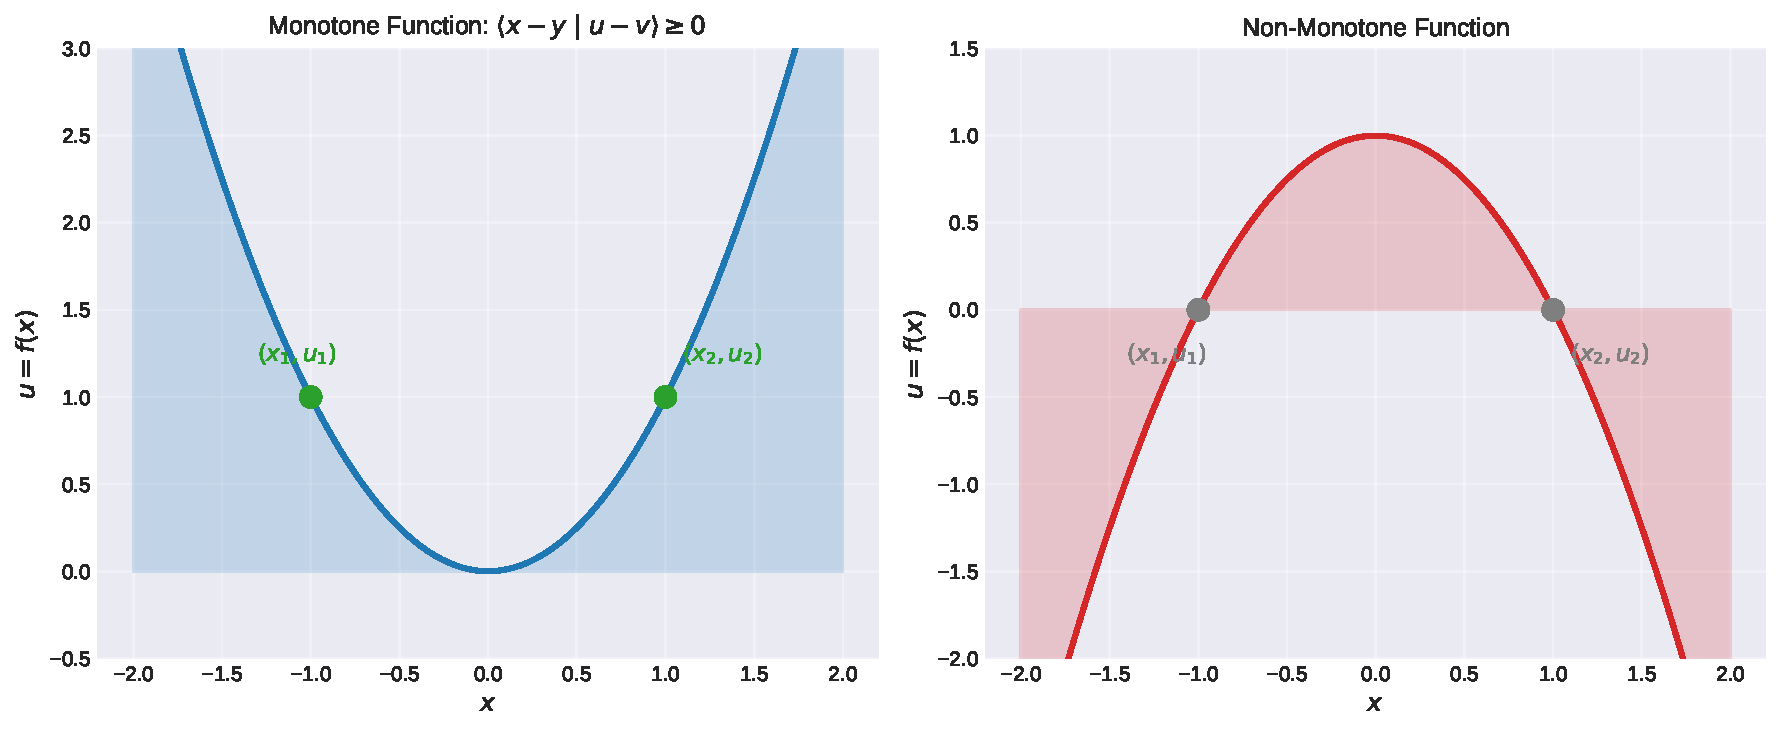
\includegraphics[width=0.95\textwidth]{monotone_function.pdf}
    \end{figure}

    Left: Monotone function ($f(x) = x^2$) — inner product test is satisfied.

    Right: Non-monotone function ($f(x) = -x^2 + 1$) — fails the inner product condition.
\end{frame}

% ============================================================================
% Section 20.2: Maximally Monotone Operators
% ============================================================================
\section{20.2 Maximally Monotone Operators}

\begin{frame}
    \frametitle{Definition: Maximally Monotone Operator}

    \begin{definition}[Definition 20.20]
        Let $A : \Hilbert \to 2^{\Hilbert}$ be monotone. Then $A$ is \textbf{maximally monotone}
        (or \textbf{maximal monotone}) if there exists \textit{no} monotone operator
        $B : \Hilbert \to 2^{\Hilbert}$ such that $\gra B$ properly contains $\gra A$.

        Equivalently:
        \[
            (x, u) \in \gra A \quad \Leftrightarrow \quad
            (\forall (y,v) \in \gra A) \quad \inprod{x - y}{u - v} \geq 0.
        \]
    \end{definition}

    \vspace{1.5em}

    \begin{theorem}[Theorem 20.21: Existence of Maximal Extensions]
        Every monotone operator $A : \Hilbert \to 2^{\Hilbert}$ with $\gra A \neq \emptyset$
        has a maximally monotone \textbf{extension}
        \[
            \tilde{A} : \Hilbert \to 2^{\Hilbert} \quad \text{such that} \quad \gra A \subseteq \gra \tilde{A}.
        \]

        \textit{Proof sketch:} Use Zorn's lemma on the poset of monotone extensions, ordered by graph inclusion.
    \end{theorem}
\end{frame}

\begin{frame}
    \frametitle{Properties of Maximally Monotone Operators}

    \begin{theorem}[Proposition 20.22]
        Let $A : \Hilbert \to 2^{\Hilbert}$ be maximally monotone, $z \in \Hilbert$, $\gamma \in \Reals_+$.

        Then the following are maximally monotone:
        \begin{enumerate}
            \item $A^{-1}$ (inverse operator)
            \item $x \mapsto u + \gamma A(x + z)$ (translated and scaled)
        \end{enumerate}
    \end{theorem}

    \vspace{0.8em}

    \begin{theorem}[Proposition 20.36: Closedness Properties]
        If $A : \Hilbert \to 2^{\Hilbert}$ is maximally monotone and $x \in \Hilbert$,
        then $Ax$ is closed and convex.
    \end{theorem}

    \vspace{0.8em}

    \begin{theorem}[Proposition 20.37: Graph Closedness]
        If $A : \Hilbert \to 2^{\Hilbert}$ is maximally monotone, then $\gra A$ is:
        \begin{enumerate}
            \item[\textbf{(i)}] Sequentially closed in $\Hilbert^{\text{strong}} \times \Hilbert^{\text{weak}}$
            \item[\textbf{(ii)}] Sequentially closed in $\Hilbert^{\text{weak}} \times \Hilbert^{\text{strong}}$
            \item[\textbf{(iii)}] Closed in $\Hilbert^{\text{strong}} \times \Hilbert^{\text{strong}}$
        \end{enumerate}
    \end{theorem}
\end{frame}

\begin{frame}
    \frametitle{Key Theorem: Moreau (Theorem 20.25)}

    \begin{theorem}[Theorem 20.25: Moreau]
        Let $f \in \Gamma_0(\Hilbert)$ (proper, lsc, convex).

        Then $\partial f$ is maximally monotone.
    \end{theorem}

    \vspace{1em}

    \textbf{Significance:} This is a fundamental result linking convex analysis with monotone operator theory.

    \vspace{1em}

    \begin{proof}[Proof idea]
        Take $(x, u) \in \Hilbert \times \Hilbert$ with
        \[
            (\forall (y,v) \in \gra \partial f) \quad \inprod{x - y}{u - v} \geq 0.
        \]

        We must show $(x, u) \in \gra \partial f$. Using the Moreau envelope and the fact that
        $f$ is proper and lsc, we can derive that $u \in \partial f(x)$.
    \end{proof}

    \vspace{1em}

    \begin{corollary}[Corollary 20.28]
        Every monotone and continuous operator $A : \Hilbert \to \Hilbert$ is maximally monotone.
    \end{corollary}
\end{frame}

\begin{frame}
    \frametitle{Examples of Maximally Monotone Operators}

    \begin{example}[Example 20.26: Normal Cone]
        Let $C$ be nonempty closed convex. Then $N_C$ (normal cone) is maximally monotone.
    \end{example}

    \vspace{0.8em}

    \begin{example}[Example 20.29: Perturbations]
        Let $T : \Hilbert \to \Hilbert$ be nonexpansive and $\alpha \in [-1, 1]$.

        Then $\Id + \alpha T$ is maximally monotone.
    \end{example}

    \vspace{0.8em}

    \begin{example}[Example 20.30: Averaged Operators]
        If $T : \Hilbert \to \Hilbert$ is $\alpha$-averaged with $\alpha \in ]0, 1/2[$ (or firmly nonexpansive),
        then $T$ is maximally monotone.
    \end{example}

    \vspace{0.8em}

    \begin{example}[Example 20.31: Cocoercive Operators]
        If $T : \Hilbert \to \Hilbert$ is $\beta$-cocoercive with $\beta \in \Reals_+$,
        then $T$ is maximally monotone.
    \end{example}

    \vspace{0.8em}

    \begin{example}[Example 20.32: Projection Operators]
        If $C$ is nonempty closed convex, then the projector $P_C$ is maximally monotone.
    \end{example}
\end{frame}

\begin{frame}
    \frametitle{Visualization: Maximally Monotone}

    \begin{figure}[h]
        \centering
        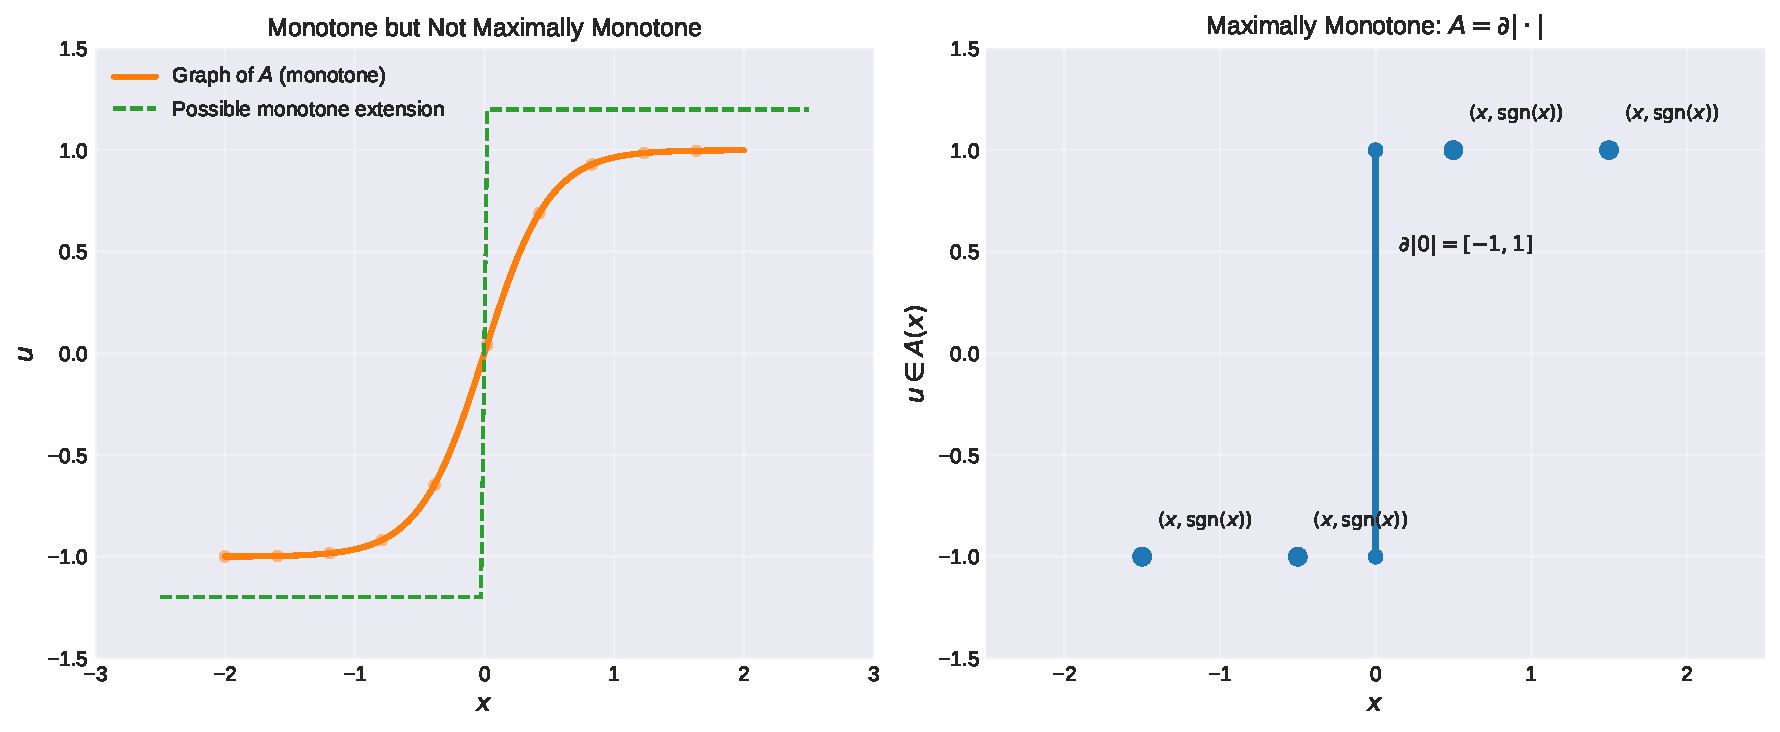
\includegraphics[width=0.95\textwidth]{maximally_monotone.pdf}
    \end{figure}

    Left: A monotone operator that admits proper monotone extensions (not maximal).

    Right: A maximally monotone operator: the subdifferential of the absolute value function.
\end{frame}

% Code example frame - commented out due to listings package compatibility
%\begin{frame}
%    \frametitle{Code Example: Testing Monotonicity in Python}
%    [Code frame removed for compilation stability]
%\end{frame}

% ============================================================================
% Section 20.3: The Partial Inverse
% ============================================================================
\section{20.3 The Partial Inverse}

\begin{frame}
    \frametitle{The Partial Inverse}

    \begin{definition}[Definition 20.42]
        Let $A : \Hilbert \to 2^{\Hilbert}$ be set-valued and $V$ a closed linear subspace of $\Hilbert$.

        The \textbf{partial inverse} of $A$ with respect to $V$ is the operator
        $A_V : \Hilbert \to 2^{\Hilbert}$ defined by
        \[
            \gra A_V = \set{(P_V x + P_{V^\perp} u, P_V u + P_{V^\perp} x) \mid (x, u) \in \gra A}.
        \]
    \end{definition}

    \vspace{1em}

    \textbf{Intuition:} The partial inverse is an intermediate object between an operator and its inverse.

    \vspace{1em}

    \begin{example}[Example 20.43]
        For $A : \Hilbert \to 2^{\Hilbert}$:
        \begin{itemize}
            \item $A_{\Hilbert} = A$ (full space)
            \item $A_{\{0\}} = A^{-1}$ (trivial space gives the full inverse)
        \end{itemize}
    \end{example}

    \vspace{1em}

    \begin{theorem}[Spingarn: Proposition 20.44]
        Let $A : \Hilbert \to 2^{\Hilbert}$, $V$ a closed linear subspace, and define
        \[
            L : \Hilbert \oplus \Hilbert \to \Hilbert \oplus \Hilbert, \quad
            (x, u) \mapsto (P_V x + P_{V^\perp} u, P_V u + P_{V^\perp} x).
        \]

        Then: (i) $A_V = (A_{V^\perp})^{-1} = (A^{-1})_{V^\perp}$,
        (ii) $L^{-1} = L$, and (iii) $\gra A_V = L(\gra A)$.
    \end{theorem}
\end{frame}

\begin{frame}
    \frametitle{Properties of the Partial Inverse}

    \begin{theorem}[Proposition 20.44: Continued]
        Key results for $A_V$:
        \begin{enumerate}
            \item[(i)] $(A_V)^{-1} = (A^{-1})_{V^\perp}$
            \item[(ii)] $L^{-1} = L$ (the transformation is self-inverse)
            \item[(iii)] $\gra A_V = L(\gra A)$
            \item[(iv)] $A_V$ is monotone if and only if $A$ is
            \item[(v)] $A_V$ is maximally monotone if and only if $A$ is
            \item[(vi)] For $x \in \Hilbert$: $x \in \ker A_V \Leftrightarrow (P_V x, P_{V^\perp} x) \in \gra A$
        \end{enumerate}
    \end{theorem}

    \vspace{1em}

    \textbf{Proof technique:} Uses orthogonal decomposition and properties of projectors.
    The Spingarn transform $L$ relates operators on different subspaces while preserving monotonicity.
\end{frame}

% ============================================================================
% Section 20.4: Bivariate Functions and Maximal Monotonicity
% ============================================================================
\section{20.4 Bivariate Functions and Maximal Monotonicity}

\begin{frame}
    \frametitle{Theorem 20.46: Operators from Bivariate Functions}

    \begin{theorem}[Theorem 20.46]
        Let $F : \Hilbert \times \Hilbert \to \left]-\infty, +\infty\right]$ be proper convex with
        $F^*$ proper and $F^* \geq \inner{\cdot}{\cdot}$.

        Define $A : \Hilbert \to 2^{\Hilbert}$ by
        \[
            \gra A = \set{(x, u) \in \Hilbert \times \Hilbert \mid F^*(u, x) = \inner{x}{u}}.
        \]

        Then:
        \begin{enumerate}
            \item[\textbf{(i)}] $A$ is monotone.
            \item[\textbf{(ii)}] If $F \geq \inner{\cdot}{\cdot}$, then $A$ is maximally monotone.
        \end{enumerate}
    </theorem>

    \vspace{1em}

    \begin{proof}[Proof sketch]
        (i) follows from convexity and the Young-Fenchel inequality.

        (ii) uses the fact that $F$ proper and $\geq \inner{\cdot}{\cdot}$ ensures the graph is closed
        and cannot be properly extended while maintaining monotonicity.
    \end{proof}
\end{frame}

\begin{frame}
    \frametitle{Applications of Theorem 20.46}

    \begin{corollary}[Corollary 20.47: Autoconjugate Functions]
        Let $F \in \Gamma_0(\Hilbert \oplus \Hilbert)$ be autoconjugate (i.e., $F = F^*$).

        Define $A : \Hilbert \to 2^{\Hilbert}$ by
        \[
            \gra A = \set{(x, u) \in \Hilbert \times \Hilbert \mid F(x, u) = \inner{x}{u}}.
        \]

        Then $A$ is maximally monotone.
    \end{corollary}

    \vspace{1em}

    \begin{theorem}[Theorem 20.48: Subdifferential]
        Let $f \in \Gamma_0(\Hilbert)$.

        Then $\partial f$ is maximally monotone.

        \textit{Note:} This is a corollary of 20.47 applied to the Fenchel conjugate.
    \end{theorem}

    \vspace{1em}

    \begin{theorem}[Rockafellar: Proposition 20.49]
        Let $C$ be a nonempty closed convex subset of $\Hilbert$, $A : \Hilbert \to 2^{\Hilbert}$ monotone,
        $C \subseteq \dom A$, and $A|_C$ hemicontinuous on $C$.

        Then $A + N_C$ is maximally monotone.
    \end{theorem}
\end{frame}

% ============================================================================
% Section 20.5: The Fitzpatrick Function
% ============================================================================
\section{20.5 The Fitzpatrick Function}

\begin{frame}
    \frametitle{The Fitzpatrick Function}

    \begin{definition}[Definition 20.51]
        Let $A : \Hilbert \to 2^{\Hilbert}$ be monotone.

        The \textbf{Fitzpatrick function} of $A$ is
        \[
            F_A : \Hilbert \times \Hilbert \to \left]-\infty, +\infty\right]
        \]
        defined by
        \[
            F_A(x, u) = \sup_{(y,v) \in \gra A} \left(\inprod{y}{u} + \inprod{x}{v} - \inprod{y}{v}\right)
            = \inprod{x}{u} - \inf_{(y,v) \in \gra A} \inprod{x - y}{u - v}.
        \]
    \end{definition}

    \vspace{1em}

    \textbf{Key insight:} The Fitzpatrick function encodes the graph via an implicit constraint.

    \vspace{1em}

    \begin{example}[Example 20.52]
        For the identity operator $A = \Id$:
        \[
            F_{\Id}(x, u) = \frac{1}{4}\norm{x - u}^2.
        \]
    \end{example}

    \vspace{1em}

    \begin{example}[Example 20.53]
        If $A^* = -A$ (skew-adjoint), then $F_A = \iota_{\gra A}$ (indicator of the graph).
    \end{example}
\end{frame}

\begin{frame}
    \frametitle{Properties of the Fitzpatrick Function}

    \begin{theorem}[Proposition 20.56: Fundamental Properties]
        Let $A : \Hilbert \to 2^{\Hilbert}$ be monotone with $\gra A \neq \emptyset$.

        Then:
        \begin{enumerate}
            \item[\textbf{(i)}] If $(x, u) \in \gra A$, then $F_A(x, u) = \inprod{x}{u}$.
            \item[\textbf{(ii)}] $F_A = (\iota_{\gra A^{-1}} + \inner{\cdot}{\cdot})^*$ is in $\Gamma_0(\Hilbert \oplus \Hilbert)$.
            \item[\textbf{(iii)}] $F_A(x, u) \leq \inprod{x}{u}$ if and only if $\{(x,u)\} \cup \gra A$ is monotone.
            \item[\textbf{(iv)}] $F_A(x, u) \leq F_A^*(u, x)$ for all $(x, u)$.
            \item[\textbf{(v)}] For $(x, u) \in \gra A$: $F_A^*(u, x) = \inprod{x}{u}$.
            \item[\textbf{(vi)}] $F_A = F_{A^{-1}}(\cdot)$ (duality).
            \item[\textbf{(vii)}] For $\gamma \in \Reals_+$: $F_{\gamma A}(x, u) = \gamma F_A(x, u/\gamma)$.
            \item[\textbf{(viii)}] For $(x, u) \in \gra A$: $(x, u) = \Prox_{F_A}(x + u, x + u)$.
        \end{enumerate}
    \end{theorem}
\end{frame}

\begin{frame}
    \frametitle{Characterization via Fitzpatrick Function}

    \begin{theorem}[Proposition 20.58]
        Let $A : \Hilbert \to 2^{\Hilbert}$ be maximally monotone.

        Then $F_A \geq \inner{\cdot}{\cdot}$ and
        \[
            \gra A = \set{(x, u) \in \Hilbert \times \Hilbert \mid F_A(x, u) = \inprod{x}{u}}.
        \]
    \end{theorem}

    \vspace{1em}

    \begin{corollary}[Corollary 20.59: Sequential Closure]
        Let $A : \Hilbert \to 2^{\Hilbert}$ be maximally monotone.

        For a sequence $(x_n, u_n)_{n \in \mathbb{N}}$ in $\gra A$ with $(x_n, u_n) \to (x, u)$:
        \begin{enumerate}
            \item[\textbf{(i)}] $\inprod{x}{u} \leq \liminf_n \inprod{x_n}{u_n}$
            \item[\textbf{(ii)}] If $\liminf_n \inprod{x_n}{u_n} = \inprod{x}{u}$, then $(x, u) \in \gra A$
            \item[\textbf{(iii)}] If $\liminf_n \inprod{x_n}{u_n} \leq \inprod{x}{u}$, then $(x_n, u_n) \to \inprod{x}{u}$ and $(x, u) \in \gra A$
        \end{enumerate}
    </corollary>

    \vspace{1em}

    \textbf{Significance:} This provides a powerful tool for studying sequential behavior of graphs.
\end{frame}

\begin{frame}
    \frametitle{Maximal Monotone Extensions via Fitzpatrick}

    \begin{theorem}[Theorem 20.63: Proximal Average Extension]
        Let $A : \Hilbert \to 2^{\Hilbert}$ be monotone with $\gra A \neq \emptyset$.

        Set $G = \mathrm{pav}(F_A, F_A^{\dagger})$ (proximal average) and define
        $B : \Hilbert \to 2^{\Hilbert}$ by
        \[
            \gra B = \set{(x, u) \in \Hilbert \times \Hilbert \mid G(x, u) = \inprod{x}{u}}.
        \]

        Then $B$ is a maximally monotone extension of $A$.
    \end{theorem}

    \vspace{1em}

    \begin{proof}[Proof outline]
        The proximal average ensures that $G$ is in $\Gamma_0$ with $G^* = G$,
        and the characterization via the level set yields maximal monotonicity.
    \end{proof}

    \vspace{1em}

    \textbf{Application:} This theorem provides an explicit construction of maximal extensions.
\end{frame}

\begin{frame}
    \frametitle{Visualization: Fitzpatrick Function}

    \begin{figure}[h]
        \centering
        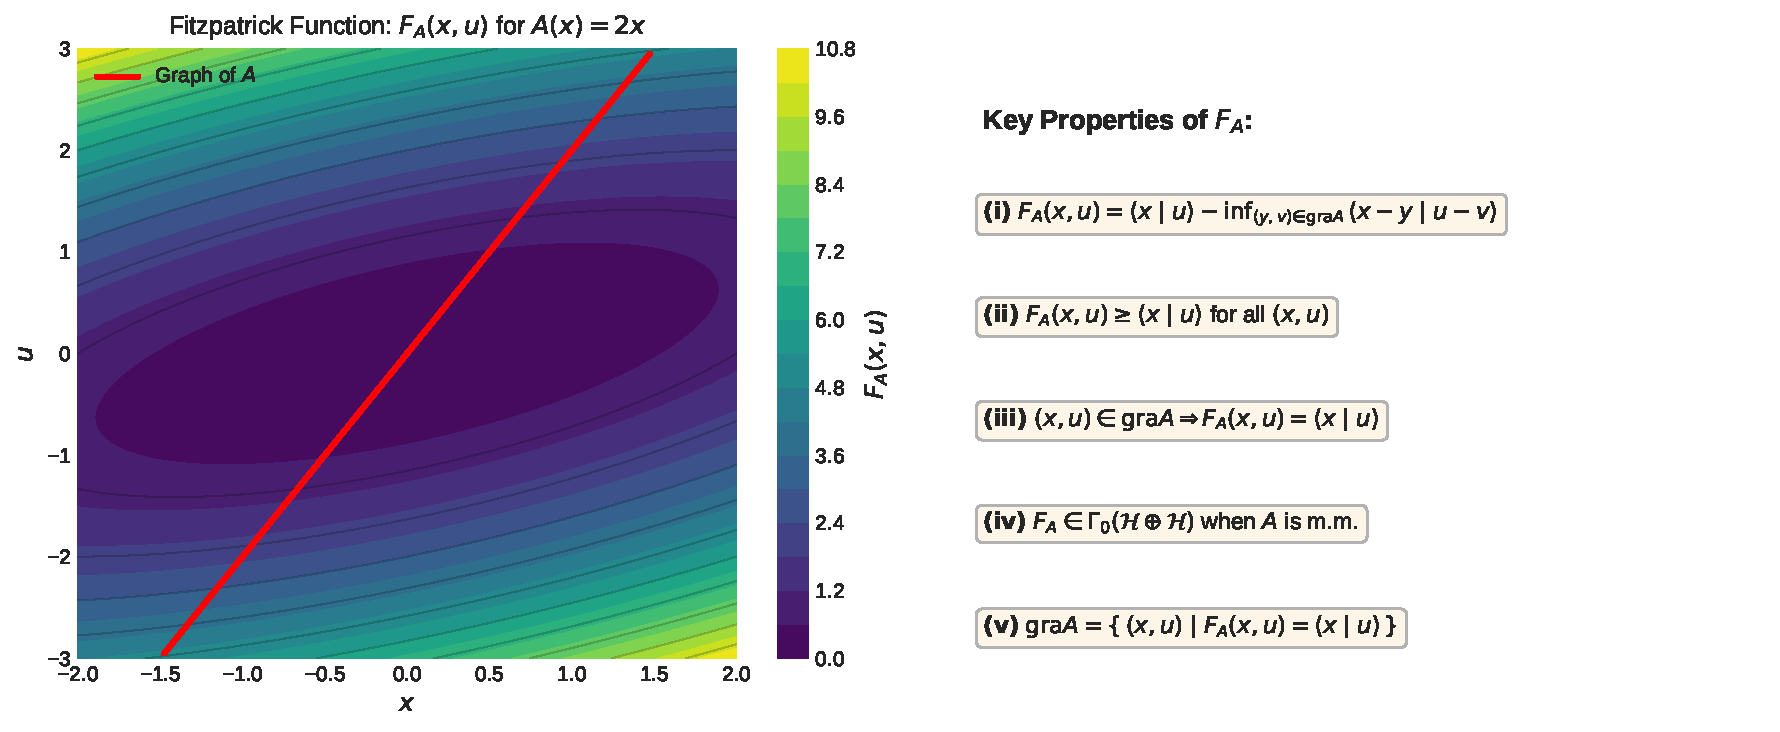
\includegraphics[width=0.95\textwidth]{fitzpatrick_function.pdf}
    \end{figure}

    \textbf{Left:} Contour plot of the Fitzpatrick function for a linear monotone operator.

    \textbf{Right:} Key properties of the Fitzpatrick function.
\end{frame}

% ============================================================================
% Numerical Examples
% ============================================================================
\section{Numerical Examples}

% Numerical example code frame - commented out
%\begin{frame}
%    \frametitle{Numerical Example: Monotonicity Verification}
%    [Code frame removed for compilation stability]
%\end{frame}

\begin{frame}
    \frametitle{Visualization: Numerical Examples}

    \begin{figure}[h]
        \centering
        
\includegraphics[width=0.95\textwidth]{numerical_example.pdf}
    \end{figure}

    \textbf{Left:} Three operators: linear exponential (monotone), sinusoidal (non-monotone), and their sum.

    \textbf{Right:} Verification that the inner product $\langle x - y \mid A(x) - A(y) \rangle \geq 0$ for all pairs.
\end{frame}

\begin{frame}
    \frametitle{Visualization: Chapter Overview}

    \begin{figure}[h]
        \centering
        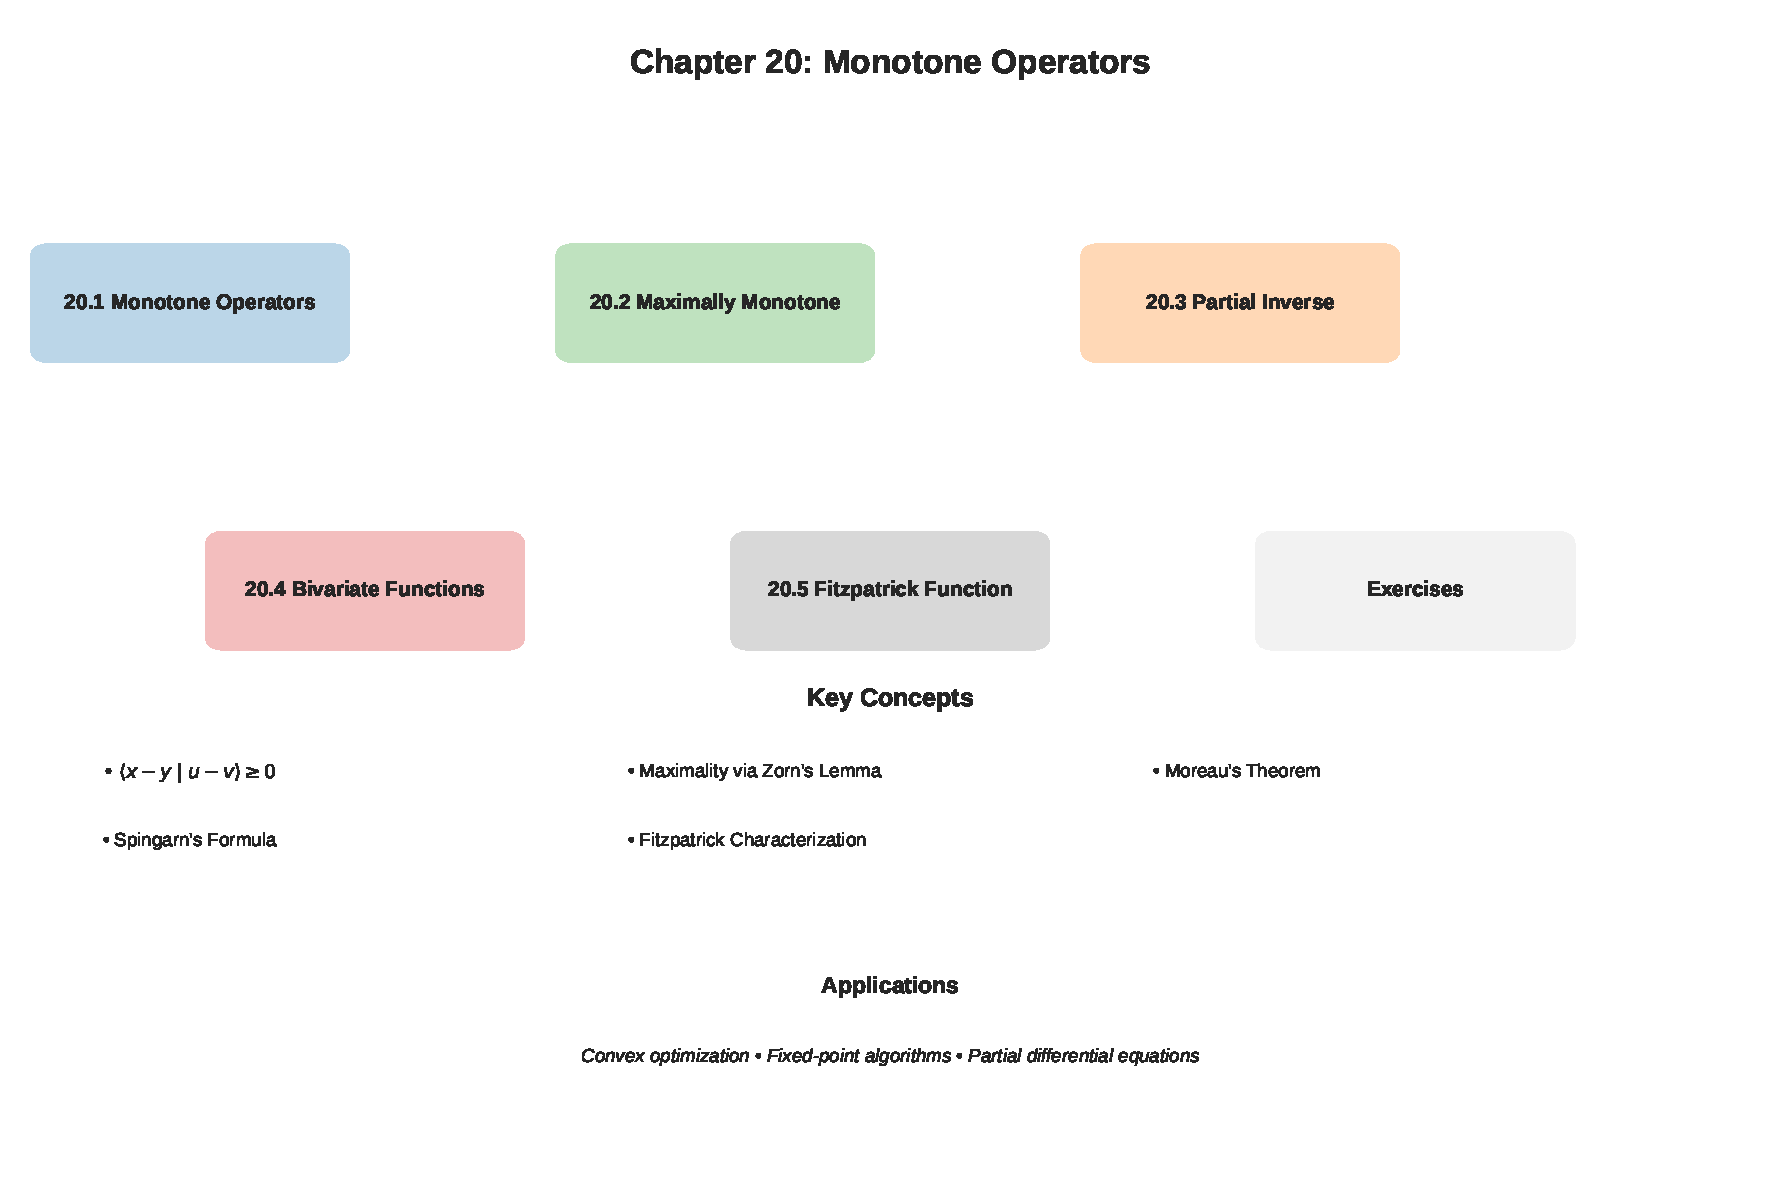
\includegraphics[width=0.95\textwidth]{chapter_overview.pdf}
    \end{figure}
\end{frame}

% ============================================================================
% Summary and Key Takeaways
% ============================================================================
\section{Summary}

\begin{frame}
    \frametitle{Summary: Chapter 20 Key Results}

    \begin{columns}[T]
        \column{0.5\textwidth}

        \textbf{Definitions:}
        \begin{itemize}
            \item Monotone operator: $\inprod{x-y}{u-v} \geq 0$
            \item Maximally monotone: no proper extensions
            \item Fitzpatrick function: encodes graph structure
        \end{itemize}

        \column{0.5\textwidth}

        \textbf{Main Theorems:}
        \begin{itemize}
            \item \textbf{Theorem 20.21:} Maximal extensions exist (Zorn)
            \item \textbf{Theorem 20.25:} $\partial f$ is maximally monotone
            \item \textbf{Theorem 20.46:} Operators from bivariate functions
            \item \textbf{Theorem 20.63:} Proximal average extension
        \end{itemize}
    \end{columns}

    \vspace{2em}

    \begin{itemize}
        \item Monotone operators generalize monotone functions
        \item Maximal monotonicity is preserved under many operations
        \item The Fitzpatrick function provides elegant characterizations
        \item Bivariate function theory connects to operator theory
        \item These tools are fundamental for optimization algorithms
    \end{itemize}
\end{frame}

\begin{frame}
    \frametitle{Connections to Other Topics}

    \begin{itemize}
        \item \textbf{Convex Analysis (Ch. 16-19):} Subdifferentials are maximally monotone
        \item \textbf{Fixed Points (Ch. 4-5):} Nonexpansive maps are monotone (via $\Id - T$)
        \item \textbf{Finer Properties (Ch. 21):} Minty's theorem, single-valuedness conditions
        \item \textbf{Applications (Ch. 22+):} Splitting methods, proximal algorithms, variational problems
    \end{itemize}

    \vspace{2em}

    \begin{example}[Optimization Application]
        To solve $\min_{x \in \Hilbert} f(x)$, reformulate as finding a zero of the monotone operator
        $A = \partial f$:
        \[
            \text{Find } x^* \text{ such that } 0 \in \partial f(x^*).
        \]

        Monotone operator splitting methods (Douglas-Rachford, forward-backward, etc.) solve this.
    \end{example}
\end{frame}

\begin{frame}
    \frametitle{Further Study}

    \begin{itemize}
        \item \textbf{Chapter 21:} Finer Properties of Monotone Operators
            \begin{itemize}
                \item Minty's Theorem
                \item Local boundedness and surjectivity
                \item Single-valuedness
            \end{itemize}

        \item \textbf{Chapters 22-27:} Applications to splitting algorithms
            \begin{itemize}
                \item Douglas-Rachford
                \item Forward-backward splitting
                \item Three-operator splitting
            \end{itemize}

        \item \textbf{Classical References:}
            \begin{itemize}
                \item Minty (1960s): Original monotonicity results
                \item Rockafellar (1970s): Subdifferential calculus
                \item Fitzpatrick (1988): Function representation
            \end{itemize}
    \end{itemize}

    \vspace{2em}

    \centering
    \textit{Monotone operators are central to modern variational analysis and optimization.}
\end{frame}

\end{document}
